Tunnistautumispalvelimella ja yksittäisellä sovelluksella on joku yhteinen salaisuus (yksityinen ja julkinen avain), jonka avulla tunnistautumispalvelin allekirjoittaa valtuutuksia (token), jolla käyttäjä voi todistaa identiteettinsä. Tähän periaatteeseen perustuvia protokollia on ainakin OAuth ja SAML. Kerberos oli tässä alunperin mukana, mutta kyseessä on matalamman tason protokolla. Ehkä sen voisi mainita? Tunnistautumispalikka voi nimittäin olla yhteydessä LDAP:in esim Kerberoksella, vaikka rajapinta käyttäjälle on OAuth (tai SAML).

Joku kiva kuva (sekvenssikaavio?), joka visualisoi asian.

\begin{figure}[ht]
\centering
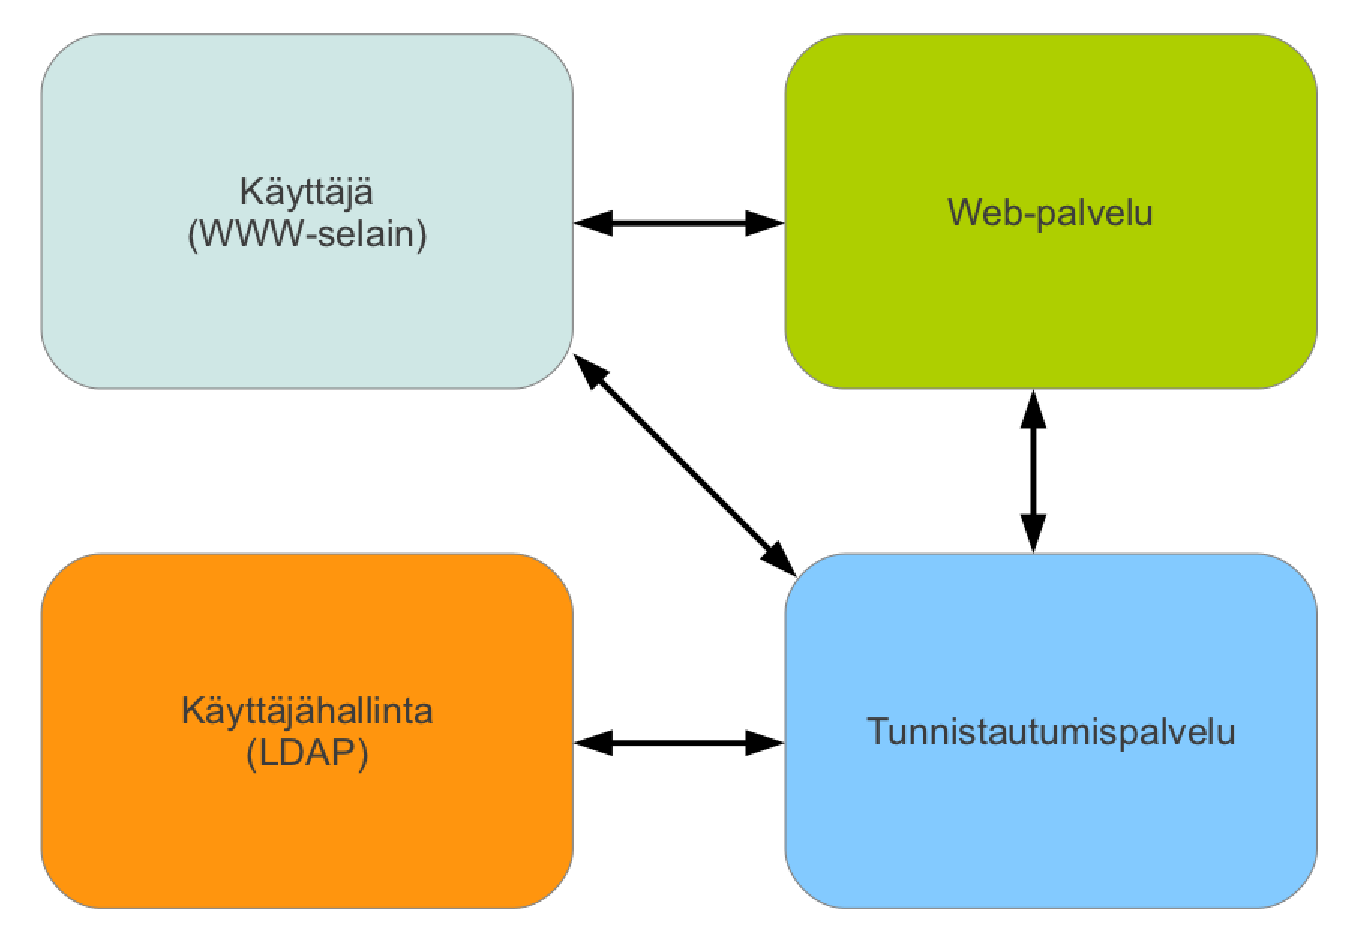
\includegraphics[width=\textwidth]{teknologiat/composition.eps}
\caption{Keskitetyn tunnistautumisen periaatteet}%
\label{composition}
\end{figure}
